% Este archivo es una biblioteca de derivaciones. Cada bloque se inserta en el
% lugar del cuerpo donde se usa, mediante \HAFOderivationpart. No se imprime
% como apéndice independiente.
\ifnum\HAFOderivationpart=1\relax
\subsection{Descomposición lineal y no lineal del campo}
\label{app:verificacion_lure}

Sea \(h(x)=\ell x+\psi(x)\). La primera ecuación de los dos modelos es
\[
{}^{\mathrm C}D_{t_0}^{q}x
=\alpha(y-x-h(x)).
\]
Al distribuir \(\alpha\),
\begin{align}
\alpha(y-x-h(x))
&=\alpha y-\alpha x-\alpha\ell x-\alpha\psi(x)\nonumber\\
&=-\alpha(1+\ell)x+\alpha y-\alpha\psi(x).
\label{eq:expansion_primera_fila}
\end{align}
Por otra parte,
\[
PX=
\begin{pmatrix}
-\alpha(1+\ell)x+\alpha y\\
x-y+z\\
-\beta y-\gamma z
\end{pmatrix},
\qquad
b\psi(r^{\T}X)=
\begin{pmatrix}
-\alpha\psi(x)\\0\\0
\end{pmatrix}.
\]
La suma reproduce \cref{eq:expansion_primera_fila} y las otras dos
ecuaciones. Para la saturación se toma
\(\ell=m_1\) y
\(\psi=(m_0-m_1)\operatorname{sat}\); para la arctangente,
\(\ell=a_1\) y \(\psi=a_2\arctan(\rho\,\cdot)\).

\fi
\ifnum\HAFOderivationpart=2\relax
\subsection{Determinante de la resolvente y transferencia}
\label{app:transferencia_explicita}

Con \(\lambda=s^q\),
\begin{equation}
\lambda I-P=
\begin{pmatrix}
\lambda+\alpha(1+\ell)&-\alpha&0\\
-1&\lambda+1&-1\\
0&\beta&\lambda+\gamma
\end{pmatrix}.
\label{eq:matriz_resolvente}
\end{equation}
El menor de la posición \((1,1)\) es
\begin{align}
Q(\lambda)
&=
\det
\begin{pmatrix}
\lambda+1&-1\\
\beta&\lambda+\gamma
\end{pmatrix}\nonumber\\
&=(\lambda+1)(\lambda+\gamma)+\beta.
\label{eq:menor_Q}
\end{align}
Al desarrollar \(\det(\lambda I-P)\) por la primera fila,
\begin{align}
\Delta_\ell(\lambda)
&=\bigl[\lambda+\alpha(1+\ell)\bigr]Q(\lambda)
-(-\alpha)
\det
\begin{pmatrix}
-1&-1\\
0&\lambda+\gamma
\end{pmatrix}\nonumber\\
&=\bigl[\lambda+\alpha(1+\ell)\bigr]Q(\lambda)
-\alpha(\lambda+\gamma).
\label{eq:determinante_transferencia}
\end{align}

Para calcular la primera componente de
\((\lambda I-P)^{-1}b\), la regla de Cramer sustituye la primera columna de
\cref{eq:matriz_resolvente} por
\(b=(-\alpha,0,0)^{\T}\). El determinante del numerador es
\[
\det
\begin{pmatrix}
-\alpha&-\alpha&0\\
0&\lambda+1&-1\\
0&\beta&\lambda+\gamma
\end{pmatrix}
=-\alpha Q(\lambda).
\]
Como \(r^{\T}\) selecciona esa primera componente,
\begin{equation}
W_q(s)
=r^{\T}(s^qI-P)^{-1}b
=-\alpha\frac{Q(s^q)}{\Delta_\ell(s^q)}.
\label{eq:transferencia_cramer}
\end{equation}

La identidad
\[
P-s^qI=-(s^qI-P)
\]
implica
\[
r^{\T}(P-s^qI)^{-1}b=-W_q(s).
\]
Por ello, cambiar el orden de los términos dentro de la resolvente cambia
simultáneamente el signo de la transferencia y el signo del cierre. No cambia
la solución física si ambas modificaciones se realizan de manera coherente.

\fi
\ifnum\HAFOderivationpart=3\relax
\subsection{Equilibrios y reducción escalar}
\label{app:equilibrios}

Para obtener los equilibrios escribimos primero el campo común a los tres
casos de Chua. Con \(X=(x,y,z)^{\T}\), sea
\[
F(X)=
\begin{pmatrix}
F_1(x,y,z)\\ F_2(x,y,z)\\ F_3(x,y,z)
\end{pmatrix}
=
\begin{pmatrix}
\alpha\bigl(y-x-h(x)\bigr)\\
x-y+z\\
-\beta y-\gamma z
\end{pmatrix}.
\]
Aquí \(h=f\) en el Chua entero, \(h=f_{\mathrm{ns}}\) en su versión
fraccionaria no suave y \(h=h_{\mathrm a}\) en el sistema con arctangente.
Por tanto, \(h\) representa la función no lineal completa que aparece dentro
del paréntesis de la primera ecuación; incluye también el término lineal
\(m_1x\) o \(a_1x\), según el modelo.

Un equilibrio es una solución constante \(X(t)=e=(x_e,y_e,z_e)^{\T}\).
La derivada ordinaria de una constante es cero y su derivada de Caputo
también lo es: para \(0<q<1\), el integrando contiene la derivada de esa
constante. En consecuencia, tanto el sistema entero como el fraccionario
exigen \(F(e)=0\), es decir,
\[
\begin{aligned}
0&=\alpha\bigl(y_e-x_e-h(x_e)\bigr),\\
0&=x_e-y_e+z_e,\\
0&=-\beta y_e-\gamma z_e.
\end{aligned}
\]
El orden \(q\) no aparece en estas ecuaciones algebraicas: cambia la dinámica
alrededor de un equilibrio, pero no su posición cuando el campo y sus
parámetros se mantienen fijos.

En todos los casos considerados, \(\alpha\neq0\) y
\(\beta+\gamma\neq0\). Comenzamos por las dos últimas ecuaciones,
\[
0=x_e-y_e+z_e,\qquad
0=-\beta y_e-\gamma z_e.
\]
De \(x_e-y_e+z_e=0\) despejamos
\[
z_e=y_e-x_e.
\]
Al sustituir este resultado en \(-\beta y_e-\gamma z_e=0\),
\begin{align*}
0
&=-\beta y_e-\gamma(y_e-x_e)\\
&=-(\beta+\gamma)y_e+\gamma x_e.
\end{align*}
Pasamos el término \(\gamma x_e\) al otro lado y dividimos por
\(\beta+\gamma\):
\[
(\beta+\gamma)y_e=\gamma x_e,
\qquad y_e=\frac{\gamma}{\beta+\gamma}x_e.
\]
Después,
\[
z_e=y_e-x_e
=\left(\frac{\gamma}{\beta+\gamma}-1\right)x_e
=\frac{\gamma-\beta-\gamma}{\beta+\gamma}x_e
=-\frac{\beta}{\beta+\gamma}x_e.
\]
Las dos coordenadas quedan expresadas en función de \(x_e\):
\begin{equation}
y_e=\frac{\gamma}{\beta+\gamma}x_e,\qquad
z_e=-\frac{\beta}{\beta+\gamma}x_e.
\label{eq:equilibrios_yz}
\end{equation}
Para usar la primera ecuación de equilibrio dividimos por \(\alpha\),
\[
0=y_e-x_e-h(x_e).
\]
Sustituimos ahora \(y_e\) y agrupamos los términos que multiplican a \(x_e\):
\begin{align*}
0
&=\frac{\gamma}{\beta+\gamma}x_e-x_e-h(x_e)\\
&=\left(\frac{\gamma}{\beta+\gamma}
       -\frac{\beta+\gamma}{\beta+\gamma}\right)x_e-h(x_e)\\
&=-\frac{\beta}{\beta+\gamma}x_e-h(x_e).
\end{align*}
Al multiplicar toda la igualdad por \(-1\), obtenemos
\begin{equation}
h(x_e)+\frac{\beta}{\beta+\gamma}x_e=0.
\label{eq:equilibrio_escalar_comun}
\end{equation}
Así se obtiene la \cref{eq:equilibrio_escalar_comun} a partir de las tres
ecuaciones originales. Para abreviar los cálculos siguientes definimos
\[
\kappa=\frac{\beta}{\beta+\gamma},
\qquad
G(x)=h(x)+\kappa x.
\]
Resolver \(G(x_e)=0\) equivale a encontrar las intersecciones de la curva
\(h(x)\) con la recta \(-\kappa x\). Cada raíz determina el punto
\[
e(x_e)=x_e
\begin{pmatrix}1\\ \gamma/(\beta+\gamma)\\-\kappa\end{pmatrix}.
\]
La construcción es suficiente, además de necesaria: al sustituir este punto
en \(F_2\) y \(F_3\), ambos se anulan por las identidades anteriores, mientras
que \(F_1(e)=-\alpha G(x_e)=0\). No se pierde ninguna ecuación al reducir
el problema a una sola incógnita.

\subsubsection{Equilibrios del Chua no suave}

La definición de la saturación permite escribir la función completa sin
dejar implícita ninguna de sus tres expresiones:
\[
h(x)=m_1x+(m_0-m_1)\operatorname{sat}(x)
=\begin{cases}
m_1x-(m_0-m_1),&x<-1,\\
m_0x,&-1\leq x\leq1,\\
m_1x+(m_0-m_1),&x>1.
\end{cases}
\]
En efecto, cuando \(-1\leq x\leq1\), la suma
\(m_1x+(m_0-m_1)x\) se reduce a \(m_0x\). Para \(x>1\) sustituimos
\(\operatorname{sat}(x)=1\), y para \(x<-1\) sustituimos
\(\operatorname{sat}(x)=-1\).

Si \(-1\leq x_e\leq1\), al introducir \(h(x_e)=m_0x_e\) en
la \cref{eq:equilibrio_escalar_comun} resulta
\begin{equation}
\left(m_0+\frac{\beta}{\beta+\gamma}\right)x_e=0.
\label{eq:equilibrio_interior_ns}
\end{equation}
Con los parámetros nominales,
\[
\kappa=\frac{12.0732}{12.0732+0.0052}
\simeq0.9995694794,
\qquad m_0+\kappa\simeq0.8227694794\neq0.
\]
Dividir por ese coeficiente da \(x_e=0\). Entonces
\(y_e=\gamma\,0/(\beta+\gamma)=0\) y
\(z_e=-\beta\,0/(\beta+\gamma)=0\); el equilibrio es \(E_0=(0,0,0)\).

Para \(x_e>1\),
\[
h(x_e)=m_1x_e+(m_0-m_1),
\]
y la \cref{eq:equilibrio_escalar_comun} queda
\[
\left(m_1+\frac{\beta}{\beta+\gamma}\right)x_e+(m_0-m_1)=0.
\]
Despejamos \(x_e\) mediante
\[
(m_1+\kappa)x_e=-(m_0-m_1)=m_1-m_0.
\]
Puesto que \(m_1+\kappa\neq0\) en este caso, la raíz positiva candidata es
\begin{equation}
x_\star=
\frac{m_1-m_0}
{m_1+\dfrac{\beta}{\beta+\gamma}}.
\label{eq:raiz_exterior_ns}
\end{equation}
Su valor y la comprobación del intervalo usado son
\[
x_\star=
\frac{-1.1468-(-0.1768)}{-1.1468+0.9995694794\ldots}
=\frac{-0.9700}{-0.1472305206\ldots}
\simeq6.5883078865>1.
\]
Para \(x_e<-1\), la ecuación correspondiente es, explícitamente,
\[
(m_1+\kappa)x_e-(m_0-m_1)=0,
\qquad
x_e=\frac{m_0-m_1}{m_1+\kappa}=-x_\star.
\]
Esta raíz satisface \(-x_\star<-1\). La pareja también se explica por la
imparidad de \(h\), pero el despeje muestra qué expresión se ha utilizado
para cada signo. Al recuperar las otras coordenadas,
\begin{equation}
E_0=(0,0,0),\qquad
E_\pm=
\left(
\pm x_\star,\,
\pm\frac{\gamma}{\beta+\gamma}x_\star,\,
\mp\frac{\beta}{\beta+\gamma}x_\star
\right).
\label{eq:equilibrios_ns_simbolicos}
\end{equation}
Por ejemplo, para \(E_+\),
\begin{align*}
y_+&=\frac{0.0052}{12.0784}(6.5883078865\ldots)
     \simeq0.0028364023,\\
z_+&=-\frac{12.0732}{12.0784}(6.5883078865\ldots)
     \simeq-6.5854714843.
\end{align*}
Por tanto, \(E_-=-E_+\). Estos equilibrios son comunes al Chua entero de
referencia y al Chua fraccionario no suave, pues ambos usan el mismo campo.

La comprobación de los intervalos forma parte de la solución: una raíz
calculada con la fórmula de \(x>1\) sólo es válida si realmente satisface
\(x>1\). Tampoco quedan equilibrios por comprobar en \(x=\pm1\), porque
\(G(1)=m_0+\kappa\neq0\) y \(G(-1)=-G(1)\neq0\).
Las divisiones anteriores se apoyan en los valores no nulos de
\(m_0+\kappa\) y \(m_1+\kappa\). Si el primero se anulara, todos los puntos
\(e(x)\) con \(-1\leq x\leq1\) serían equilibrios; si el segundo se anulara,
habría que resolver la ecuación constante de cada intervalo exterior antes
de usar la \cref{eq:raiz_exterior_ns}. Ninguna de estas degeneraciones ocurre
con los parámetros estudiados.

\subsubsection{Equilibrios del Chua con arctangente}

Al usar
\(h(x)=a_1x+a_2\arctan(\rho x)\) en
la \cref{eq:equilibrio_escalar_comun}, se obtiene
\begin{equation}
\left(a_1+\frac{\beta}{\beta+\gamma}\right)x_e
+a_2\arctan(\rho x_e)=0.
\label{eq:equilibrio_escalar_arctan}
\end{equation}
Definimos \(c=a_1+\kappa\), de modo que la función cuya raíz buscamos es
\[
G(x)=cx+a_2\arctan(\rho x).
\]
Como \(G(-x)=-G(x)\), el origen siempre es raíz y las raíces no nulas
aparecen por parejas. La simetría por sí sola no demuestra que existan
tres equilibrios. Para establecer su número calculamos
\[
G'(x)=c+\frac{a_2\rho}{1+\rho^2x^2},
\qquad
G''(x)=-\frac{2a_2\rho^3x}{(1+\rho^2x^2)^2}.
\]
En los dos conjuntos de parámetros, \(c>0\), \(a_2<0\), \(\rho>0\) y
\(G'(0)=c+a_2\rho<0\). Por ello, \(G\) decrece inmediatamente a la derecha
del origen. Además, \(G''(x)>0\) para \(x>0\), por lo que su pendiente
aumenta estrictamente hasta tender a \(c>0\). El único mínimo positivo se
obtiene haciendo \(G'(x)=0\):
\begin{align*}
\frac{a_2\rho}{1+\rho^2x^2}&=-c,\\
1+\rho^2x^2&=-\frac{a_2\rho}{c},\\
x_{\min}&=\frac{1}{\rho}
\sqrt{-\frac{a_2\rho}{c}-1}.
\end{align*}
Así, \(G(x_{\min})<0\). Después del mínimo la función crece estrictamente y
tiende a \(+\infty\), ya que \(cx\) crece sin cota y la arctangente permanece
acotada. Existe, por tanto, una única raíz positiva \(x_\star\), una negativa
\(-x_\star\) y la raíz cero.

Para calcular \(x_\star\) disponemos de un intervalo explícito. Sea
\[
B=-\frac{a_2\pi}{2c}>0.
\]
Entonces
\[
G(B)=-a_2\left[\frac{\pi}{2}-\arctan(\rho B)\right]>0,
\qquad G(x_{\min})<0.
\]
La raíz queda entre \(x_{\min}\) y \(B\). Se puede obtener por bisección en
ese intervalo o por el método de Newton,
\[
x_{n+1}=x_n-
\frac{cx_n+a_2\arctan(\rho x_n)}
{c+a_2\rho/(1+\rho^2x_n^2)},
\]
con \(x_0=B\). Como \(G\) es convexa y creciente entre \(x_\star\) y \(B\),
los iterados de Newton descienden hacia la raíz dentro de ese intervalo.
No se inicia en \(x_{\min}\), donde \(G'\) se anula y el cociente no está
definido. Los valores de los extremos para cada caso son
\[
\begin{array}{c|rrrr}
\text{Caso}&c&G'(0)&x_{\min}&B\\ \hline
\text{Wu}&1.39956948&-0.15893052&0.33698178&1.74917081\\
\texttt{c590}&1.04190329&-4.95905111&1.21309002&5.03060522
\end{array}
\]
Se usa \(\rho=1\) para Wu y \(\rho=1.7984259333\) para \texttt{c590}.
Con los parámetros escritos en las \cref{eq:parametros_wu,eq:parametros_c590},
la sustitución de las raíces positivas en la \cref{eq:equilibrios_yz} da
\[
\begin{array}{c|rrr}
\text{Caso}&x_\star&y_+&z_+\\ \hline
\text{Wu}&0.60967912&0.00026248&-0.60941664\\
\texttt{c590}&4.64940551&0.00179700&-4.64760851
\end{array}
\]
Por ejemplo, en Wu,
\[
y_+=\frac{0.0052}{12.0784}(0.6096791169\ldots),
\qquad
z_+=-\frac{12.0732}{12.0784}(0.6096791169\ldots).
\]
En \texttt{c590}, los mismos despejes usan
\(\beta+\gamma=19.0892188529\) y la raíz \(4.6494055136\ldots\).
En ambos casos, \(E_0=(0,0,0)\), \(E_+=(x_\star,y_+,z_+)\) y
\(E_-=-E_+\). Las coordenadas mostradas están redondeadas; la ecuación
\(G(x_\star)=0\) y la reconstrucción de \(y_+,z_+\) se evalúan antes de ese
redondeo.

\begin{figure}[htbp]
\centering
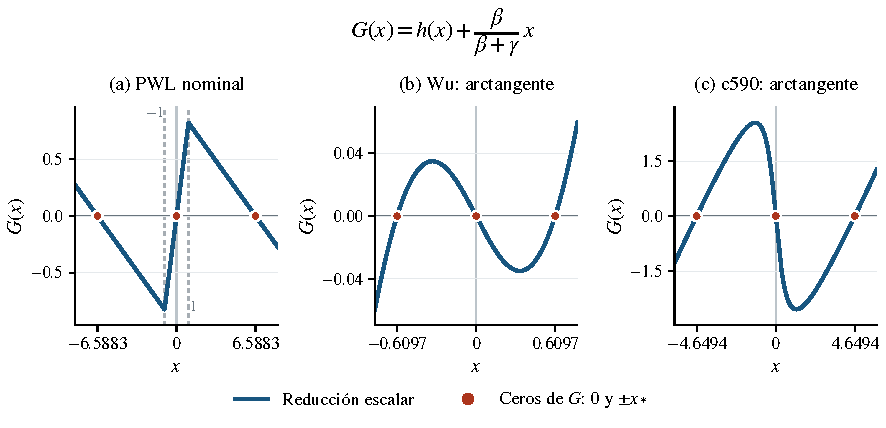
\includegraphics[width=0.98\textwidth]{figures/fundamentos/equilibrios_reduccion_escalar.pdf}
\caption{Reducción del cálculo de equilibrios a los ceros de
\(G(x)=h(x)+\kappa x\). Cada cero proporciona una coordenada \(x_e\), a partir
de la cual se recuperan \(y_e\) y \(z_e\). Las líneas verticales del caso
no suave señalan los cambios de expresión de \(h\) en \(x=\pm1\).}
\label{fig:equilibrios_reduccion_escalar}
\end{figure}
\FloatBarrier

\fi
\ifnum\HAFOderivationpart=4\relax
\subsection{Cálculo del jacobiano en cada equilibrio}
\label{app:jacobianos}

El jacobiano describe cómo cambia el campo cuando desplazamos ligeramente
el estado. Sus filas corresponden a las tres ecuaciones del sistema y sus
columnas a las variables \(x,y,z\). Por definición,
\[
DF(X)=
\begin{pmatrix}
\partial F_1/\partial x&\partial F_1/\partial y&\partial F_1/\partial z\\
\partial F_2/\partial x&\partial F_2/\partial y&\partial F_2/\partial z\\
\partial F_3/\partial x&\partial F_3/\partial y&\partial F_3/\partial z
\end{pmatrix}.
\]
Para construirlo partimos directamente de las ecuaciones del campo, antes
de evaluar cualquier equilibrio. En la primera componente distribuimos
\(\alpha\):
\[
F_1=\alpha y-\alpha x-\alpha h(x).
\]
Al derivar respecto de \(x\), mantenemos \(y,z\) constantes; al derivar
respecto de \(y\), mantenemos \(x,z\) constantes. De ahí,
\[
\frac{\partial F_1}{\partial x}=-\alpha-\alpha h'(x)
=-\alpha[1+h'(x)],\qquad
\frac{\partial F_1}{\partial y}=\alpha,\qquad
\frac{\partial F_1}{\partial z}=0.
\]
Para \(F_2=x-y+z\), las tres derivadas son
\[
\frac{\partial F_2}{\partial x}=1,\qquad
\frac{\partial F_2}{\partial y}=-1,\qquad
\frac{\partial F_2}{\partial z}=1.
\]
Finalmente, \(F_3=-\beta y-\gamma z\) no depende de \(x\), y por tanto
\[
\frac{\partial F_3}{\partial x}=0,\qquad
\frac{\partial F_3}{\partial y}=-\beta,\qquad
\frac{\partial F_3}{\partial z}=-\gamma.
\]
Una vez calculadas las nueve entradas, sustituimos \(X=e\). El jacobiano
evaluado en el equilibrio es
\begin{equation}
J(e)=DF(e)=
\begin{pmatrix}
-\alpha[1+h'(x_e)]&\alpha&0\\
1&-1&1\\
0&-\beta&-\gamma
\end{pmatrix}.
\label{eq:jacobiano_lure}
\end{equation}
Sólo la entrada de la primera fila y primera columna depende de la posición
del equilibrio. Esto ocurre porque \(h\) depende únicamente de \(x\) y las
otras dos ecuaciones son lineales.

Para interpretar la matriz, escribimos un estado cercano como
\(X=e+\xi\), donde \(\xi=(\xi_x,\xi_y,\xi_z)^{\T}\) es una perturbación.
La expansión de Taylor del campo alrededor de \(e\) da
\[
F(e+\xi)=F(e)+J(e)\xi+R(\xi),
\qquad \frac{\lVert R(\xi)\rVert}{\lVert\xi\rVert}\longrightarrow0
\quad\text{cuando }\xi\longrightarrow0.
\]
Como \(F(e)=0\) y la derivada de la constante \(e\) se anula, la ecuación de
la perturbación es
\[
{}^{\mathrm C}D_{t_0}^{q}\xi=J(e)\xi+R(\xi),
\]
o \(\dot\xi=J(e)\xi+R(\xi)\) en el caso entero. Al conservar los términos
de primer orden obtenemos el sistema lineal
\[
\begin{aligned}
{}^{\mathrm C}D_{t_0}^{q}\xi_x
 &=-\alpha[1+h'(x_e)]\xi_x+\alpha\xi_y,\\
{}^{\mathrm C}D_{t_0}^{q}\xi_y
 &=\xi_x-\xi_y+\xi_z,\\
{}^{\mathrm C}D_{t_0}^{q}\xi_z
 &=-\beta\xi_y-\gamma\xi_z.
\end{aligned}
\]
Esta es la función del jacobiano: proporciona el sistema que gobierna las
perturbaciones pequeñas alrededor de un equilibrio determinado.

\subsubsection{Jacobianos del Chua no suave en \(E_0\), \(E_+\) y \(E_-\)}

La función \(h\) es afín entre sus puntos de cambio de pendiente. Al
derivar cada expresión obtenida en el apartado anterior,
\[
h'(x)=
\begin{cases}
m_1,&x<-1,\\
m_0,&-1<x<1,\\
m_1,&x>1.
\end{cases}
\]
Los números \(-1\) y \(1\) señalan dónde cambia la fórmula de \(h\).
Estos intervalos pertenecen a la definición de la función; no representan
cuencas de atracción ni clasifican por sí mismos una trayectoria.
Para calcular \(J(e)\) basta identificar en cuál de los intervalos está
la coordenada \(x_e\) del equilibrio que se está estudiando.

En \(E_0\), \(x_e=0\), así que \(h'(0)=m_0\). En \(E_+\),
\(x_e=x_\star>1\), por lo que \(h'(x_\star)=m_1\). En \(E_-\),
\(x_e=-x_\star<-1\), y también \(h'(-x_\star)=m_1\). Sustituir estas
pendientes en la \cref{eq:jacobiano_lure} produce
\begin{equation}
\begin{aligned}
J(E_0)&=
\begin{pmatrix}
-\alpha(1+m_0)&\alpha&0\\
1&-1&1\\
0&-\beta&-\gamma
\end{pmatrix},\\[2mm]
J(E_+)=J(E_-)&=
\begin{pmatrix}
-\alpha(1+m_1)&\alpha&0\\
1&-1&1\\
0&-\beta&-\gamma
\end{pmatrix}.
\end{aligned}
\label{eq:jacobianos_ns}
\end{equation}
Los dos equilibrios no nulos tienen la misma matriz porque la pendiente
es \(m_1\) en ambos. Los términos constantes \(\pm(m_0-m_1)\), que sí
intervienen al localizar \(E_\pm\), desaparecen al derivar.

Con los valores nominales, la primera entrada se calcula como
\[
-\alpha(1+m_0)=-8.4562(1-0.1768)=-6.96114384,
\]
\[
-\alpha(1+m_1)=-8.4562(1-1.1468)=1.24137016.
\]
Por tanto, las matrices concretas son
\[
\begin{aligned}
J(E_0)&=
\begin{pmatrix}
-6.96114384&8.4562&0\\
1&-1&1\\
0&-12.0732&-0.0052
\end{pmatrix},\\[2mm]
J(E_+)=J(E_-)&=
\begin{pmatrix}
1.24137016&8.4562&0\\
1&-1&1\\
0&-12.0732&-0.0052
\end{pmatrix}.
\end{aligned}
\]
En este modelo la expansión lineal es exacta mientras la coordenada
perturbada \(x_e+\xi_x\) permanezca en el mismo intervalo que \(x_e\):
allí \(R(\xi)=0\), porque el campo es afín. Basta que \(|\xi_x|<1\) alrededor
de \(E_0\), o que \(|\xi_x|<x_\star-1\) alrededor de \(E_+\) y \(E_-\).
En \(x=\pm1\), las pendientes
laterales son distintas para \(m_0\neq m_1\) y no existe una derivada clásica
única. Ninguno de los tres equilibrios nominales está en esos puntos.

\subsubsection{Jacobianos del Chua con arctangente en los tres equilibrios}

La derivada de la arctangente se calcula mediante la regla de la cadena:
\[
\frac{\mathrm d}{\mathrm dx}\arctan(\rho x)
=\frac{1}{1+(\rho x)^2}\frac{\mathrm d(\rho x)}{\mathrm dx}
=\frac{\rho}{1+\rho^2x^2}.
\]
Por consiguiente, para la función completa \(h(x)=a_1x+a_2\arctan(\rho x)\),
\[
h'(x)=a_1+\frac{a_2\rho}{1+\rho^2x^2}.
\]
Al evaluar esta pendiente en \(x=x_e\),
\begin{equation}
J(e)=
\begin{pmatrix}
\displaystyle
-\alpha\left(1+a_1+
\frac{a_2\rho}{1+\rho^2x_e^2}\right)
&\alpha&0\\[3mm]
1&-1&1\\
0&-\beta&-\gamma
\end{pmatrix}.
\label{eq:jacobiano_arctan}
\end{equation}
En el origen y en los dos equilibrios no nulos, respectivamente,
\[
h'(0)=a_1+a_2\rho,
\qquad
h'(x_\star)=h'(-x_\star)
=a_1+\frac{a_2\rho}{1+\rho^2x_\star^2}.
\]
La igualdad entre las dos últimas pendientes se debe al cuadrado
\(x_\star^2\); así, también en esta familia \(J(E_+)=J(E_-)\).
Por ejemplo, para Wu,
\[
h'(0)=0.4-1.5585=-1.1585,
\qquad
h'(x_\star)=0.4-
\frac{1.5585}{1+(0.6096791169\ldots)^2}.
\]
Para \texttt{c590}, la sustitución es
\[
\begin{aligned}
h'(0)&=0.0422897934-3.3367815123(1.7984259333),\\
h'(x_\star)&=0.0422897934-
\frac{3.3367815123(1.7984259333)}
{1+(1.7984259333)^2(4.6494055136\ldots)^2}.
\end{aligned}
\]
Cada uno de estos valores se introduce en la entrada
\(-\alpha[1+h'(x_e)]\) de la primera fila. Las otras ocho entradas son las
ya calculadas; se usan los parámetros \(\alpha,\beta,\gamma\) del mismo
caso. Los resultados numéricos de esa sustitución son
\[
\begin{array}{c|rrrr}
\text{Caso}&h'(0)&h'(x_\star)&[J(E_0)]_{11}&[J(E_\pm)]_{11}\\ \hline
\text{Wu}&-1.15850000&-0.73617424&1.34030770&-2.23096342\\
\texttt{c590}&-5.95866461&-0.04233015&108.34363289&-20.92447026
\end{array}
\]
Por ejemplo, la primera fila de \(J(E_0)\) para Wu es
\((1.34030770,\,8.4562,\,0)\), mientras que la de \(J(E_+)\) es
\((-2.23096342,\,8.4562,\,0)\); las dos filas restantes coinciden con las
de las matrices no suaves nominales porque comparten \(\beta,\gamma\).
En \texttt{c590}, la segunda fila sigue siendo \((1,-1,1)\), la tercera
es \((0,-19.0818408409,-0.0073780120)\) y la entrada \((1,2)\) es
\(\alpha=21.8493569066\).

La función con arctangente es suave en todo \(\mathbb R\), por lo que
el jacobiano existe en cualquier estado y \(R(\xi)=O(\lVert\xi\rVert^2)\)
alrededor de cada equilibrio.

\subsubsection{Valores propios y estabilidad local}

Un valor propio \(\lambda\) de \(J(e)\) satisface
\[
J(e)v=\lambda v,\qquad v\neq0.
\]
El vector \(v\) identifica un modo de perturbación del sistema lineal.
En el sistema entero, ese modo evoluciona mediante \(e^{\lambda t}\):
su amplitud disminuye cuando \(\operatorname{Re}\lambda<0\) y aumenta
cuando \(\operatorname{Re}\lambda>0\). La matriz puede tener valores propios
complejos, que describen modos oscilatorios junto con su crecimiento o
decrecimiento. La estabilidad se determina con los valores propios, no con
el signo de una sola entrada del jacobiano.

Para \(q=1\), el sistema lineal de perturbaciones es asintóticamente estable
si y sólo si sus tres valores propios tienen parte real negativa. Para el
sistema lineal de Caputo con orden común \(0<q<1\), el criterio de
Matignon~\cite{Matignon1996} establece la condición
\[
\lambda_j\neq0,\qquad
|\arg\lambda_j|>\frac{q\pi}{2},\qquad j=1,2,3.
\]
Aquí \(\arg\lambda_j\in(-\pi,\pi]\) es el ángulo del valor propio en el
plano complejo, medido desde el semieje real positivo. El criterio exige
que los tres valores propios queden fuera del sector de apertura \(q\pi\)
centrado en ese semieje. Cuando \(q=1\), la condición angular recupera el
semiplano de parte real negativa. Para \(0<q<1\), los modos de perturbación
fraccionarios siguen funciones de Mittag--Leffler y su decaimiento está
determinado por ese sector angular.

Esta condición clasifica la aproximación lineal y, bajo las hipótesis de
linealización, establece la estabilidad local del equilibrio. Si un valor
propio está exactamente en la frontera angular, el criterio estricto no
decide el comportamiento del sistema no lineal. El jacobiano describe la
dinámica próxima a cada equilibrio; la localización de otros atractores y
sus cuencas requiere las trayectorias del sistema completo.

\fi
\ifnum\HAFOderivationpart=5\relax
\subsection{Polinomio característico y coeficientes}
\label{app:polinomio_caracteristico}

Sea \(g=h'(x_e)\) la pendiente total de la no linealidad en un equilibrio.
El jacobiano de cualquiera de las dos familias puede escribirse como
\begin{equation}
J(g)=
\begin{pmatrix}
-\alpha(1+g)&\alpha&0\\
1&-1&1\\
0&-\beta&-\gamma
\end{pmatrix}.
\label{eq:jacobiano_pendiente_total}
\end{equation}
Por tanto,
\[
\lambda I-J(g)=
\begin{pmatrix}
\lambda+\alpha(1+g)&-\alpha&0\\
-1&\lambda+1&-1\\
0&\beta&\lambda+\gamma
\end{pmatrix}.
\]
Los valores propios son las raíces de
\(\chi_g(\lambda)=\det[\lambda I-J(g)]\). Desarrollamos el determinante
aquí, con los signos \(+,-,+\) de los cofactores de la primera fila:
\begin{align*}
\chi_g(\lambda)
={}&[\lambda+\alpha(1+g)]
\det\begin{pmatrix}\lambda+1&-1\\\beta&\lambda+\gamma\end{pmatrix}\\
&-(-\alpha)
\det\begin{pmatrix}-1&-1\\0&\lambda+\gamma\end{pmatrix}.
\end{align*}
El tercer término es cero porque la entrada \((1,3)\) es cero. Los dos
determinantes de orden dos se calculan como producto de la diagonal
principal menos producto de la otra diagonal:
\[
\begin{aligned}
\det\begin{pmatrix}\lambda+1&-1\\\beta&\lambda+\gamma\end{pmatrix}
&=(\lambda+1)(\lambda+\gamma)-(-1)\beta\\
&=(\lambda+1)(\lambda+\gamma)+\beta,\\[1mm]
\det\begin{pmatrix}-1&-1\\0&\lambda+\gamma\end{pmatrix}
&=(-1)(\lambda+\gamma)-(-1)0\\
&=-(\lambda+\gamma).
\end{aligned}
\]
Por ello, el segundo cofactor aporta
\(-(-\alpha)[-(\lambda+\gamma)]=-\alpha(\lambda+\gamma)\).
Al reunir ambos términos,
\begin{equation}
\chi_g(\lambda)
=\bigl[\lambda+\alpha(1+g)\bigr]
\bigl[(\lambda+1)(\lambda+\gamma)+\beta\bigr]
-\alpha(\lambda+\gamma).
\label{eq:polinomio_caracteristico_agrupado}
\end{equation}
Para expandir el resultado, primero multiplicamos los dos binomios:
\[
(\lambda+1)(\lambda+\gamma)+\beta
=\lambda^2+\gamma\lambda+\lambda+\gamma+\beta
=\lambda^2+(1+\gamma)\lambda+(\beta+\gamma).
\]
Escribiendo temporalmente \(A=\alpha(1+g)\), la multiplicación completa es
\begin{align*}
\chi_g(\lambda)
={}&(\lambda+A)
\bigl[\lambda^2+(1+\gamma)\lambda+(\beta+\gamma)\bigr]
-\alpha\lambda-\alpha\gamma\\
={}&\lambda^3+(1+\gamma)\lambda^2+(\beta+\gamma)\lambda\\
&+A\lambda^2+A(1+\gamma)\lambda+A(\beta+\gamma)
-\alpha\lambda-\alpha\gamma\\
={}&\lambda^3+[1+\gamma+A]\lambda^2\\
&+[\beta+\gamma+A(1+\gamma)-\alpha]\lambda
+A(\beta+\gamma)-\alpha\gamma.
\end{align*}
Finalmente sustituimos \(A=\alpha(1+g)\) y factorizamos \(\alpha\) en el
término independiente:
\begin{equation}
\begin{aligned}
\chi_g(\lambda)
={}&\lambda^3+
\bigl[1+\gamma+\alpha(1+g)\bigr]\lambda^2\\
&+\bigl[
\beta+\gamma+\alpha(1+g)(1+\gamma)-\alpha
\bigr]\lambda\\
&+\alpha\bigl[(1+g)(\beta+\gamma)-\gamma\bigr].
\end{aligned}
\label{eq:polinomio_caracteristico_expandido}
\end{equation}
En el sistema no suave se sustituye \(g=m_0\) en \(E_0\) y \(g=m_1\)
en \(E_\pm\). En el sistema con arctangente,
\[
g=a_1+\frac{a_2\rho}{1+\rho^2x_e^2}.
\]
Cada sustitución proporciona un polinomio cúbico concreto. Sus tres raíces
son los valores propios del jacobiano en el equilibrio correspondiente.
Con ellos se aplica el criterio de estabilidad expuesto al final de
la \cref{app:jacobianos}, usando el orden \(q\) del mismo caso de estudio.

\fi
\ifnum\HAFOderivationpart=6\relax
\subsection{Primer armónico de la saturación centrada}
\label{app:df_saturacion_centrada}

Sea
\[
\psi_{\mathrm{ns}}(\sigma)=\Delta\operatorname{sat}(\sigma),
\qquad \Delta=m_0-m_1.
\]
Si \(0<A\leq1\), no hay saturación y
\[
\psi_{\mathrm{ns}}(A\sin\theta)=\Delta A\sin\theta.
\]
Como \(\int_0^\pi\sin^2\theta\dd\theta=\pi/2\),
\[
N_{\mathrm{ns}}(A)
=\frac{2}{\pi A}\Delta A\frac{\pi}{2}
=\Delta.
\]

Para \(A>1\), defínase
\[
\theta_0=\arcsin\left(\frac1A\right),
\qquad 0<\theta_0<\frac{\pi}{2}.
\]
En \(0\leq\theta\leq\theta_0\) y
\(\pi-\theta_0\leq\theta\leq\pi\), la entrada permanece en la parte lineal;
en el intervalo central la saturación vale \(1\). Entonces
\begin{align}
N_{\mathrm{ns}}(A)
&=\frac{2\Delta}{\pi A}
\left[
2A\int_0^{\theta_0}\sin^2\theta\dd\theta
+\int_{\theta_0}^{\pi-\theta_0}\sin\theta\dd\theta
\right]\nonumber\\
&=\frac{2\Delta}{\pi A}
\left[
A\theta_0-\frac{A}{2}\sin(2\theta_0)
+2\cos\theta_0
\right]\nonumber\\
&=\frac{2\Delta}{\pi A}
\left[A\theta_0+\cos\theta_0\right].
\label{eq:df_sat_pasos}
\end{align}
En el último paso se usó
\[
\frac{A}{2}\sin(2\theta_0)
=A\sin\theta_0\cos\theta_0
=\cos\theta_0.
\]
Finalmente,
\[
\cos\theta_0
=\sqrt{1-\frac1{A^2}}
=\frac{\sqrt{A^2-1}}{A},
\]
y \cref{eq:df_sat_pasos} se convierte en
\[
N_{\mathrm{ns}}(A)
=\Delta\frac{2}{\pi}
\left[
\arcsin\left(\frac1A\right)
+\frac{\sqrt{A^2-1}}{A^2}
\right],
\]
La unión de las dos ramas es continua en \(A=1\), pues
\(\arcsin(1)=\pi/2\) y \(\sqrt{A^2-1}\to0\). Para estudiar su rango,
derivamos los dos términos de la rama saturada:
\[
 \frac{\dd}{\dd A}\arcsin(A^{-1})=-\frac1{A\sqrt{A^2-1}},
 \qquad
 \frac{\dd}{\dd A}\frac{\sqrt{A^2-1}}{A^2}
 =\frac1{A\sqrt{A^2-1}}-\frac{2\sqrt{A^2-1}}{A^3}.
\]
Los primeros términos se cancelan y obtenemos
\begin{equation}
 N'_{\mathrm{ns}}(A)=-\frac{4\Delta\sqrt{A^2-1}}{\pi A^3},
 \qquad A>1.
 \label{eq:df-saturacion-rango-derivada}
\end{equation}
Si \(\Delta>0\), \(N_{\mathrm{ns}}\) decrece de \(\Delta\) a cero en
esa rama; si \(\Delta<0\), crece de \(\Delta\) a cero. En ambos casos
el cierre tiene una única amplitud \(A>1\) cuando la ganancia está
estrictamente entre esos extremos. La ganancia \(k=\Delta\) corresponde
a todo \(0<A\leq1\), por lo que allí el balance fundamental no selecciona
una amplitud aislada. Esto precisa tanto \cref{eq:df_saturacion} como su
uso para construir semillas.

\fi
\ifnum\HAFOderivationpart=7\relax
\subsection{Media y primer armónico de la saturación sesgada}
\label{app:df_saturacion_sesgada}

Considérese
\[
u(\theta)=c+A\cos\theta,\qquad A>0.
\]
Para escribir una fórmula que incluya los casos parcialmente y completamente
saturados, se define
\[
[v]_{-1}^{1}=\max(-1,\min(1,v))
\]
y los ángulos
\begin{equation}
\theta_+
=\arccos\left[\frac{1-c}{A}\right]_{-1}^{1},
\qquad
\theta_-
=\arccos\left[\frac{-1-c}{A}\right]_{-1}^{1}.
\label{eq:angulos_saturacion_sesgada}
\end{equation}
Como \((1-c)/A>(-1-c)/A\) y \(\arccos\) es decreciente,
\(0\leq\theta_+\leq\theta_-\leq\pi\). En el intervalo
\([0,\pi]\),
\[
\operatorname{sat}(u(\theta))=
\begin{cases}
1,&0\leq\theta\leq\theta_+,\\
c+A\cos\theta,&\theta_+\leq\theta\leq\theta_-,\\
-1,&\theta_-\leq\theta\leq\pi.
\end{cases}
\]
La simetría respecto de \(2\pi\) permite integrar solamente en
\([0,\pi]\). Para \(\psi=\Delta\operatorname{sat}\),
\begin{align}
\Psi_0(c,A)
=\frac{\Delta}{\pi}\Big[
&\theta_+
+c(\theta_--\theta_+)
+A(\sin\theta_--\sin\theta_+)\nonumber\\
&-(\pi-\theta_-)
\Big].
\label{eq:psi0_saturacion_cerrada}
\end{align}

Para la componente fundamental se usan
\[
\int\cos\theta\dd\theta=\sin\theta,\qquad
\int\cos^2\theta\dd\theta
=\frac{\theta}{2}+\frac{\sin2\theta}{4}.
\]
La sustitución por intervalos da
\begin{align}
\Psi_1(c,A)
=\frac{2\Delta}{\pi}\Bigg[
&\sin\theta_++\sin\theta_-
+c(\sin\theta_--\sin\theta_+)\nonumber\\
&+\frac{A}{2}(\theta_--\theta_+)
+\frac{A}{4}
\bigl(\sin2\theta_--\sin2\theta_+\bigr)
\Bigg].
\label{eq:psi1_saturacion_cerrada}
\end{align}
Las operaciones de recorte en
\cref{eq:angulos_saturacion_sesgada} hacen que
\cref{eq:psi0_saturacion_cerrada,eq:psi1_saturacion_cerrada} sigan siendo
válidas cuando alguna de las tres regiones tiene longitud cero.

La ecuación de media puede reducirse a una igualdad escalar. De
\cref{eq:transferencia_cramer},
\begin{align}
W_q(0)
&=-\alpha
\frac{\beta+\gamma}
{\alpha(1+\ell)(\beta+\gamma)-\alpha\gamma}\nonumber\\
&=-\frac{\beta+\gamma}
{(1+\ell)(\beta+\gamma)-\gamma}.
\label{eq:ganancia_dc}
\end{align}
Por tanto,
\begin{equation}
c=W_q(0)\Psi_0(c,A),
\label{eq:cierre_dc_escalar}
\end{equation}
y el cierre armónico es
\[
1-W_q(\ii\omega)\frac{\Psi_1(c,A)}{A}=0.
\]
Estas tres ecuaciones reales ---una para la media, y las partes real e
imaginaria del cierre--- determinan \((c,A,\omega)\).

\fi
\ifnum\HAFOderivationpart=8\relax
\subsection{Integral de Fourier de la arctangente}
\label{app:df_arctan}

Sea
\[
\psi_{\mathrm a}(\sigma)=a_2\arctan(\rho\sigma),
\qquad
\xi=\rho A.
\]
Se define
\[
I(\xi)=
\int_0^\pi\arctan(\xi\sin\theta)\sin\theta\dd\theta.
\]
Como \(I(0)=0\), puede calcularse \(I\) integrando su derivada.
La diferenciación bajo la integral es válida porque el integrando y su
derivada respecto de \(\xi\) son continuos y están uniformemente
acotados en cada intervalo compacto de \(\xi\). Para \(\xi>0\),
\begin{align}
I'(\xi)
&=\int_0^\pi
\frac{\sin^2\theta}{1+\xi^2\sin^2\theta}\dd\theta\nonumber\\
&=\frac1{\xi^2}
\left[
\pi-\int_0^\pi
\frac{\dd\theta}{1+\xi^2\sin^2\theta}
\right]\nonumber\\
&=\frac{\pi}{\xi^2}
\left(1-\frac1{\sqrt{1+\xi^2}}\right).
\label{eq:derivada_integral_arctan}
\end{align}
Para justificar la última igualdad, la simetría respecto de \(\pi/2\)
reduce la integral a dos veces \([0,\pi/2]\). Con
\(u=\tan\theta\), \(\sin^2\theta=u^2/(1+u^2)\) y
\(\dd\theta=\dd u/(1+u^2)\), se obtiene
\begin{align*}
 \int_0^\pi\frac{\dd\theta}{1+\xi^2\sin^2\theta}
 &=2\int_0^\infty\frac{\dd u}{1+(1+\xi^2)u^2}\\
 &=\frac{2}{\sqrt{1+\xi^2}}
 \left[\arctan\!\left(u\sqrt{1+\xi^2}\right)\right]_0^\infty
 =\frac{\pi}{\sqrt{1+\xi^2}}.
\end{align*}
La primitiva puede comprobarse sin una integración implícita. Si
\(s=\sqrt{1+\xi^2}\), entonces
\[
 \frac{\dd}{\dd\xi}\frac{s-1}{\xi}
 =\frac{\xi^2/s-(s-1)}{\xi^2}
 =\frac{1-1/s}{\xi^2}.
\]
Además, \((s-1)/\xi=\xi/(1+s)\to0\). Multiplicar por \(\pi\)
y usar \(I(0)=0\) fija la constante de integración y produce
\begin{equation}
I(\xi)
=\pi\frac{\sqrt{1+\xi^2}-1}{\xi}.
\label{eq:integral_arctan}
\end{equation}
Al sustituir \(\xi=\rho A\) en
\cref{eq:df_centrada},
\begin{align}
N_{\mathrm a}(A)
&=\frac{2a_2}{\pi A}I(\rho A)\nonumber\\
&=\frac{2a_2}{\rho A^2}
\left(\sqrt{1+\rho^2A^2}-1\right)\nonumber\\
&=\frac{2a_2\rho}
{1+\sqrt{1+\rho^2A^2}}.
\label{eq:df_arctan_derivada}
\end{align}

Para \(\rho>0\), \(a_2\ne0\) y \(k\ne0\), si el cierre exige
\(N_{\mathrm a}(A)=k\), la amplitud puede despejarse.
De la forma racionalizada,
\[
1+\sqrt{1+\rho^2A^2}=\frac{2a_2\rho}{k}.
\]
Al aislar la raíz y elevar al cuadrado se obtiene
\[
 \rho^2A^2
 =\left(\frac{2a_2\rho}{k}-1\right)^2-1
 =\frac{4a_2^2\rho^2}{k^2}-\frac{4a_2\rho}{k}.
\]
La división entre \(\rho^2>0\) da
\begin{equation}
A^2
=\frac{4a_2(a_2\rho-k)}{k^2\rho}.
\label{eq:amplitud_arctan}
\end{equation}
La solución se acepta solamente si el lado derecho es positivo y la igualdad
previa a elevar al cuadrado tiene lado derecho mayor que \(2\). De manera
equivalente, para \(A>0\), \(k\) tiene el mismo signo que \(a_2\) y se
encuentra estrictamente entre \(0\) y \(a_2\rho\), con el orden de los
extremos ajustado al signo de \(a_2\).

\fi
\ifnum\HAFOderivationpart=9\relax
\subsection{Identidad modal y normalización de la salida}
\label{app:identidad_modal}

Sea \(P_0=P+bkr^{\T}\). Entonces
\[
\zeta I-P_0=(\zeta I-P)-bkr^{\T}.
\]
Si \(\zeta I-P\) es invertible, el lema del determinante matricial
\(\det(M+uv^{\T})=\det(M)(1+v^{\T}M^{-1}u)\), con
\[
M=\zeta I-P,\qquad u=-bk,\qquad v=r,
\]
produce
\begin{align}
\det(\zeta I-P_0)
&=\det(\zeta I-P)
\left[1-kr^{\T}(\zeta I-P)^{-1}b\right]\nonumber\\
&=\det(\zeta I-P)\bigl[1-kG(\zeta)\bigr],
\label{eq:lema_determinante_aplicado}
\end{align}
donde
\[
G(\zeta)=r^{\T}(\zeta I-P)^{-1}b,
\qquad W_q(s)=G(s^q).
\]
El producto del lado derecho tiene la expresión polinómica
\[
 \det(\zeta I-P)-k r^{\T}\operatorname{adj}(\zeta I-P)b.
\]
Esta expresión extiende la identidad a los polos; no asigna allí un valor
a la resolvente ni a \(G\). Fuera de los polos, si
\[
1-kG(\zeta_0)=0,
\]
entonces \(\det(\zeta_0I-P_0)=0\). Puede construirse directamente el
vector normalizado
\[
 v=k(\zeta_0I-P)^{-1}b.
\]
En efecto, \(r^{\T}v=kG(\zeta_0)=1\), de modo que \(v\ne0\), y
\[
 (\zeta_0I-P_0)v
 =(\zeta_0I-P)v-bkr^{\T}v=bk-bk=0.
\]
Si se obtiene primero un autovector por otro procedimiento, su proyección
\(r^{\T}v\) tampoco puede anularse: de lo contrario sería un
autovector de \(P\) en \(\zeta_0\), contradiciendo la invertibilidad
del resolvente. Por tanto, se puede dividir por esa proyección y obtener
la normalización usada en \cref{eq:modo_normalizado,eq:semilla_modal}.

Para la matriz de Chua, las dos últimas filas de
\((\zeta_0I-P_0)v=0\) no contienen \(k\). Con \(v_1=1\) son
\[
 -1+(\zeta_0+1)v_2-v_3=0,
 \qquad \beta v_2+(\zeta_0+\gamma)v_3=0.
\]
Su determinante es \(Q(\zeta_0)\). Cuando no se anula,
\begin{equation}
 v=\left(1,\frac{\zeta_0+\gamma}{Q(\zeta_0)},
              -\frac{\beta}{Q(\zeta_0)}\right)^{\T}.
 \label{eq:modo-chua-componentes-explicitas}
\end{equation}
La primera fila impone
\(\Delta_\ell(\zeta_0)+\alpha kQ(\zeta_0)=0\), exactamente
\(1-kG(\zeta_0)=0\). En una raíz finita del cierre con \(k\ne0\),
\(G(\zeta_0)=1/k\ne0\) excluye \(Q(\zeta_0)=0\); por ello esta
expresión es compatible con la construcción mediante la resolvente.

En la rama sesgada,
\[
X_1=\bigl[(\ii\omega_0)^qI-P\bigr]^{-1}b\Psi_1.
\]
Al premultiplicar por \(r^{\T}\),
\[
r^{\T}X_1
=W_q(\ii\omega_0)\Psi_1
=W_q(\ii\omega_0)N_1A.
\]
El cierre \(1-W_qN_1=0\) prueba algebraicamente que
\(r^{\T}X_1=A\).

\fi
\ifnum\HAFOderivationpart=10\relax
\subsection{Homotopía afín y conservación de la media}
\label{app:homotopia_afin}

La aproximación sesgada separa
\[
\psi(\sigma)
=\Psi_0+N_1(\sigma-c)
+\bigl[\psi(\sigma)-\Psi_0-N_1(\sigma-c)\bigr].
\]
Se definen
\begin{equation}
P_{\mathrm a}=P+N_1br^{\T},\qquad
d_{\mathrm a}=b(\Psi_0-N_1c).
\label{eq:parametros_homotopia_afin}
\end{equation}
La familia de campos es
\begin{equation}
\begin{aligned}
F_\varepsilon(X)
&=P_{\mathrm a}X+d_{\mathrm a}\\
&\quad+\varepsilon b
\left[
\psi(r^{\T}X)-\Psi_0-N_1(r^{\T}X-c)
\right],
\qquad 0\leq\varepsilon\leq1.
\end{aligned}
\label{eq:homotopia_afin}
\end{equation}

En \(\varepsilon=0\), la media \(\bar X\) de
\cref{eq:cierre_dc_sesgado} es un equilibrio del auxiliar:
\begin{align*}
F_0(\bar X)
&=P\bar X+bN_1c+b\Psi_0-bN_1c\\
&=P\bar X+b\Psi_0=0.
\end{align*}
Para una perturbación \(\xi=X-\bar X\),
\[
F_0(\bar X+\xi)=P_{\mathrm a}\xi,
\]
de modo que el auxiliar conserva tanto la media como el modo armónico.

En \(\varepsilon=1\), al agrupar términos,
\begin{align*}
F_1(X)
&=PX+bN_1r^{\T}X+b\Psi_0-bN_1c\\
&\quad+b\psi(r^{\T}X)-b\Psi_0-bN_1r^{\T}X+bN_1c\\
&=PX+b\psi(r^{\T}X).
\end{align*}
Así, el extremo final de \cref{eq:homotopia_afin} es exactamente el sistema
físico de \cref{eq:lure_comun}. Una homotopía centrada de la forma
\(P_0X+\varepsilon b[\psi(\sigma)-k\sigma]\) no conserva, en general, la
media \(c\neq0\); por eso no se utiliza para la rama sesgada.
\fi
